%%%%%%%%%%%%%%%%%%%%%%%%%%%%%%%%%%%%%%%%%%%%%%%%%%%%%%%%%%%%%%%%%%%%%%%%%%%

\documentclass{standalone}

\usepackage{amsmath}
\usepackage{mathptmx}
\usepackage{pgfplots}
\usetikzlibrary{external}
\tikzexternalize{sunflower-delta}
\pgfplotsset{compat=1.16}

%% IEEE uses Times Roman font, so we'll default to Times.
%% These three commands make up the entire times.sty package.
\renewcommand{\rmdefault}{ptm}
\renewcommand{\ttdefault}{pcr}
\normalfont\selectfont

\begin{document}

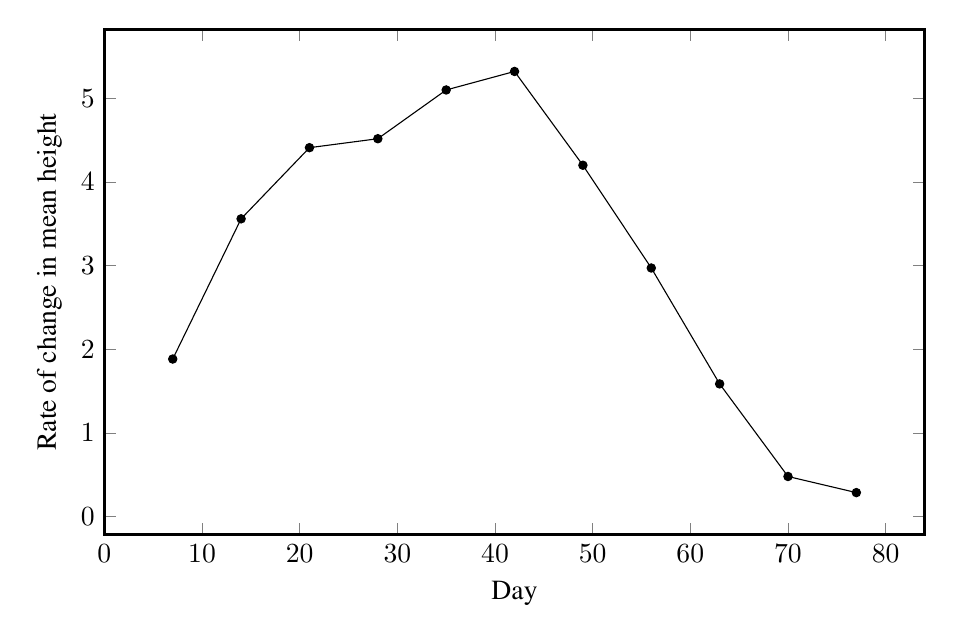
\begin{tikzpicture}
\tikzset{%%
  every mark/.append style={scale=1.0},%%
  scale=1.0%%
}
\pgfplotsset{%%
  every axis/.append style={font=\normalsize}%%
}
%%
\begin{axis}[%%
  axis line style=very thick,%%
  dotStyle/.style={mark size=1.5,black,mark color=black,mark=*},%%
  enlargelimits=true,%%
  height=8cm,%%
  width=12cm,%%
  %% x axis
  xlabel={\normalsize Day},%%
  %% y axis
  ylabel={\normalsize Rate of change in mean height}%%
]
%%
%%
\addplot[dotStyle] coordinates {
  (7, 1.88285714285714)
  (14, 3.55928571428571)
  (21, 4.41)
  (28, 4.51714285714286)
  (35, 5.1)
  (42, 5.32142857142857)
  (49, 4.2)
  (56, 2.97142857142857)
  (63, 1.58571428571429)
  (70, 0.47857142857143)
  (77, 0.285714285714286)
};
\end{axis}
\end{tikzpicture}

\end{document}
